\def\VCDate{2016/04/22}\def\VCVersion{(Current)}
\documentclass{article}
\usepackage{ProofPower,verbatim,graphicx,float}
\usepackage{amsmath,amsfonts,fpic,color,pstricks,xcolor,pstricks-add}
\usepackage{underscore,listings,hyperref}
\usepackage[margin=0.5in,paperwidth=6in,paperheight=5in]{geometry}
\title{gcd function in sml, C, and asm}
\setcounter{secnumdepth}{0}
\begin{document} 
\author{Saw Thinkar Nay Htoo}
\maketitle
\clearpage

\begin{GFT}{SML}
\+fun sqr x : real = x * x;\\
\+fun odd x = x mod 2 = 1;\\
\+fun power r p = if p = 0 then 1.0;\\
\+		else if odd p then r * power r (p-1)\\
\+		else sqr (power r (p div 2));\\
\+power 2.0 9;\\
\+\\
\end{GFT}
\begin{GFT}{C source code written to file lab4.c}
\+\#include <stdio.h>\\
\+typedef enum \{false,true\} bool;\\
\+float sqr (float x) \{return x * x;\}\\
\+bool odd(int x) \{return x \% 2 == 1;\}\\
\+float power (float r, int p)\\
\+\{\\
\+	if (p == 0) return 1.0;\\
\+	else if (odd(p)) return r * power (r,p-1);\\
\+	else return sqr (power (r,p/2));\\
\+\}\\
\+int main()\\
\+\{\\
\+	printf("\%f\Backslash{}n", power(2.0,9));\\
\+\}\\
\end{GFT}
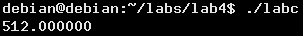
\includegraphics[scale = 0.5]{labc.png}
\clearpage\section*{ASM}
\begin{GFT}{ASM source code written to file lab4.s}
\+.equ flase,0\\
\+.equ true,1\\
\+\\
\+.data\\
\+r: .float 2.0\\
\+f: .float 0.0\\
\+fmt: .string "\%f\Backslash{}n"\\
\+\\
\end{GFT}
\clearpage\section*{Square}
\verb|float sqr (float x) {return x * x;}|
Expects x to be on the system stack, return $x^2$ in register ST(0).
\begin{enumerate}
\item load x into ST(0)
\item load x into ST(1)
\item multiply ST(1) times ST(0)

\end{enumerate}
\begin{GFT}{ASM source code appended to file lab4.s}
\+.text\\
\+sqr:\\
\+  flds 4(\%esp)\\
\+  flds 4(\%esp)\\
\+  fmul \%ST(1),\%ST(0)\\
\+  ret\\
\end{GFT}

\clearpage\section*{Odd}
\begin{GFT}{ASM source code appended to file lab4.s}
\+odd:\\
\+  ret\\
\end{GFT}

\clearpage\section*{Power}
\begin{GFT}{ASM source code appended to file lab4.s}
\+power:\\
\+ flds r\\
\+ ret\\
\+\\
\end{GFT}
\clearpage\section*{Main}
\begin{GFT}{ASM source code appended to file lab4.s}
\+.globl \_start\\
\+\\
\+\_start:\\
\+	push \$9\\
\+	push r\\
\+	call power\\
\+	add \$8, \%esp\\
\+\\
\+	fstps f\\
\+\#to try the square function\\
\+	push r \\
\+	call sqr\\
\+	add \$4, \%esp\\
\end{GFT}
\clearpage\section*{}
\begin{GFT}{ASM source code appended to file lab4.s}
\+\#to try printf - to push 64-bit vlaue instead of 32\\
\+		\\
\+	sub \$8, \%esp\\
\+	fstps (\%esp)\\
\+\\
\+	push \$fmt\\
\+	call printf\\
\+	add \$12, \%esp \#1 32-bit param, 1 64-bit param = 12 bytes\\
\end{GFT}

\clearpage\section*{Exit}
\begin{GFT}{ASM source code appended to file lab4.s}
\+	mov \$1,\%eax\\
\+	mov \$0,\%ebx\\
\+	int \$0x80\\
\end{GFT}
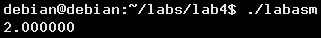
\includegraphics[scale = 0.5]{labasm.png}
\clearpage
	
\begin{GFT}{Text written to file labcode.sh}
\+docsml lab4.doc\\
\+as -gstabs -o lab.o lab4.s\\
\+ld -dynamic-linker /lib/ld-linux.so.2 -o labasm lab.o -lc -lX11\\
\+\#gcc -Wall -g -o labc lab4.c\\
\+\\
\end{GFT}
\begin{GFT}{Text written to file labcode2.sh}
\+gcc -Wall -o labc lab4.c\\
\+gcc -Wall -o labasm lab4.s\\
\+\\
\end{GFT}
\begin{GFT}{Text written to file labdoc.sh}
\+doctex lab4.doc\\
\+pptexenv /home/debian/texfot.pl pdflatex lab4.tex\\
\+\\
\end{GFT}
\begin{GFT}{Bourne Shell}
\+chmod 755 labcode2.sh\\
\+chmod 755 labcode.sh\\
\+chmod 755 labdoc.sh\\
\+\\
\end{GFT}
\end{document}
